\subsection{Emergent Fermions at the Endpoints of Strings -- Equivalence between Spin and Fermion Representation}\label{sec:Emergent-Fermions-at-the-Endpoints}
In Appendix \ref{appendix:Majorana-derivation}, we will give another way of deriving the ground state density matrix of the Kitaev model, which starts from the Majorana representation. We will see in equation \eqref{equ.Majorana-density-matrix} that the ground state density matrix can also be represented as
\[
  \rho = 2^{N-1}\mathcal{P}_G\prod_{\anglelr{ij}}\lr{\frac{\mathds{1}+\hat{u}_{ij}}{2}}\rho_F\mathcal{P}_G
\]
where $\rho_F$ is the density matrix of the Kitaev ground state in the Majorana fermion representation and $\mathcal{P}_G$ is the Gutzwiller projection \cite{burnell-nayak, projector-1, projector-2}. The Majorana density matrix $\rho_F$ can be constructed from a starting point similar to equation \eqref{equ.rho-starting} we have used at the very beginning
\begin{equation}\label{equ.rho-F}
    \rho^F = \frac{1}{2^{N/2}}\sum_{[\mathfrak{D}]}\mathfrak{C}_\mathfrak{D}\mathcal{M}_\mathfrak{D}
\end{equation}
where
\begin{equation}\label{equ.V-rep-def}
    \mathcal{M}_\mathfrak{D} \equiv \prod_{\anglelr{ij}\in\mathfrak{D}}ic_jc_i
\end{equation}
In each dimer $\anglelr{ij}$ of the above product, the site $i$ belongs to sublattice $A$ and $j$ to sublattice $B$. The denominator of the normalization coefficient is $2^{N/2}$ instead of $2^N$ because a normal fermion $f$ is defined by two $c$-Majorana fermions $c_1$ and $c_2$ as $f=\frac{1}{2}(c_1+ic_2)$ and $f^\dagger=\frac{1}{2}(c_1-ic_2)$. Therefore, the total number of physical degrees of freedom of a system composed of $N$ Majorana fermions is $2^{N/2}$ instead of $2^N$. To manifest the similarity between the spin density matrix \eqref{equ.density-matrix}, we define a set of operators $\mathcal{S}_{\mathfrak{D}}$ for each operator that corresponds to an edge configuration
\begin{equation}\label{equ.S-def}
    \mathcal{S}_\mathfrak{D} \equiv \mathcal{P}_{\mrm{topo}}\mathcal{P}^{(p)}\Sigma_\mathfrak{D}
\end{equation}
Given equation \eqref{equ.Sigma-representation} and the fact that $[\mathcal{P}_G,\Sigma_{\mathfrak{D}}]=0$, the set of operators $\lrg{\mathcal{S}_{\mathfrak{D}}}$ also forms a representation of the algebra of edge configurations $\anglelr{\lrg{\mathfrak{D}},\oplus}$, 
\begin{equation}\label{equ.U-rep-algebra}
    \mathcal{S}_{\mathfrak{D}}\mathcal{S}_{\mathfrak{D}'} = g(\mathfrak{D},\mathfrak{D}')\mathcal{S}_{\mathfrak{D}\oplus\mathfrak{D}'}.
\end{equation}
With the string representation \eqref{equ.S-def} and \eqref{equ.U-rep-algebra}, The form of the density matrix in Eq.~\eqref{equ.density-matrix} becomes
\begin{equation}\label{equ.rho-U}
    \rho =  \frac{1}{2^{N-N_p}} \sum_{[\mathfrak{D}]}\mathfrak{C}_{\mathfrak{D}}\mathcal{S}_{\mathfrak{D}}
\end{equation}
which is of a form extremely similar to \eqref{equ.rho-F} if those $\mathcal{S}$-operators are replaced by $\mathcal{M}$-operators. This is reminiscent of different representations of the same algebra.
If we use the Majorana fermions to represent spin operators as $\sigma^\mu\to ib^\mu c$, then 
\begin{align*}
    \mathcal{S}_\mathfrak{D} &\to \mathcal{P}^{(p)} \prod_{\anglelr{ij}\in \mathfrak{D}}\lr{\hat{u}_{ij}ic_jc_i} \\
    &= \mathcal{P}^{(p)} \lrm{\prod_{\anglelr{ij}\in \mathfrak{D}}\hat{u}_{ij}} \mathcal{M}_{\mathfrak{D}}
\end{align*}
The first two products completely consist of $\hat{u}_{ij}$'s, which commute with each other as well as the $c$-Majorana fermion operators~\footnote{Note that the projector $\mathcal{P}^{(p)}$ becomes
\[\mathcal{P}^{(p)} \to \prod_{ p}\lr{\frac{\mathds{1} + \prod_{\anglelr{ij}\in p}\hat{u}_{ij}}{2}}\]
in the Majorana representation, where ``$\anglelr{ij}\in p$'' stands for \textit{those edges of the plaquette $p$}.}. Therefore, they will not contribute to the phase factor $g\lr{\mathfrak{D},\mathfrak{D}'}$ at all. So, we know that the anti-commutation relations among $c$-Majorana fermions are encoded in the phase factor $g\lr{\mathfrak{D},\mathfrak{D}'}$. In view of this, we find that the set of operators $\mathcal{M}_\mathfrak{D}$ defined by equation \eqref{equ.V-rep-def} also forms a projective representation of the edge configuration algebra and shares the same phase factor $g\lr{\mathfrak{D},\mathfrak{D}'}$ with the representation $\mathcal{S}$
\begin{equation}\label{equ.V-rep-algebra}
    \mathcal{M}_{\mathfrak{D}}\mathcal{M}_{\mathfrak{D}'} = g(\mathfrak{D},\mathfrak{D}')\mathcal{M}_{\mathfrak{D}\oplus\mathfrak{D}'}
\end{equation}
This clearly illustrated a picture: the Majorana fermion representation is identical to the spin, or Pauli string, representation, and the Majorana fermions can be seen as emerging from the endpoints of those Pauli strings defined by \eqref{equ.string-operator-def}~\cite{Kitaev, fermion-and-string, string-net, Photons-and-electrons-as-emergent-phenomena-string, PRD-string-wen-quantum-order}. Remember that the core principle that allows us to describe the Kitaev model using gauge theory is the fractionalization of spin degrees of freedom into Majorana fermions and gauge fields. To analyze everything in spin language, we have to always represent everything in strings in such a way that two Majorana fermions or gauge field operators in every pair, which appear in the gauge theory after the fractionalization of the spin degrees of freedom, are connected by a string. More vividly speaking, we have to \textit{glue} those fractionalized degrees of freedom back via string operators defined in spin language. \valert{From this perspective, the fermion anticommutation relation is clearly evident in \autoref{fig.standard-configuration}. 
\begin{figure}
    \centering
    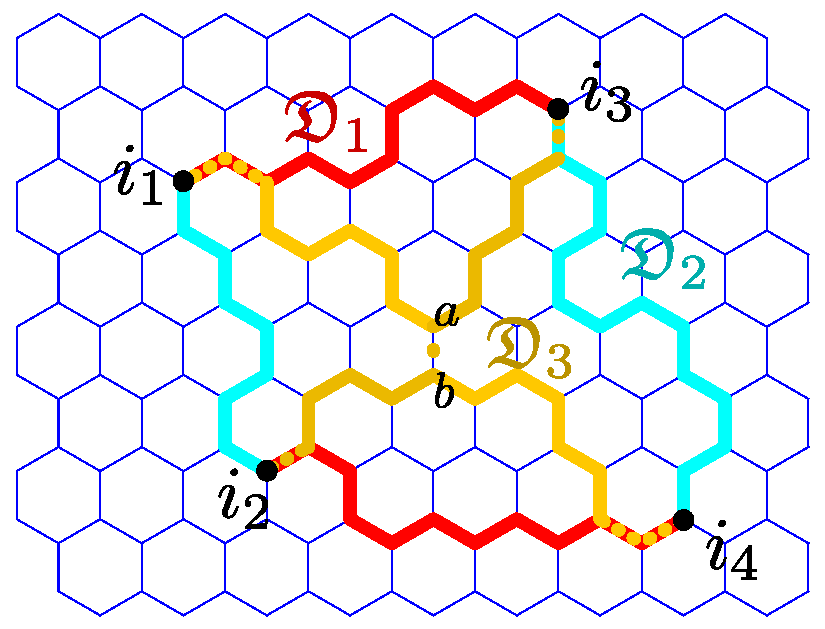
\includegraphics[width=0.7\linewidth]{figures/exchange.pdf}
    \caption{$\mathfrak{D}_1$ and $\mathfrak{D}_2$ are equivalent configurations because they share the same set of endpoints. $\mathfrak{D}_2$ can be decomposed into two strings ($\overline{i_1i_2}$ and $\overline{i_3i_4}$) that connect different types of endpoints, while $\mathfrak{D}_1$ is composed of two strings ($\overline{i_1i_3}$ and $\overline{i_2i_4}$) connecting the same type of endpoints. Another configuration $\mathfrak{D}_3$ is the combination of two strings ($\overline{i_1i_4}$ and $\overline{i_2i_3}$) connecting different types of endpoints. Still, the intersection part (brown dotted segment $\overline{ab}$ at the center of the figure) vanishes because the combination is accomplished by performing $\oplus$ between the two edge configurations, making it equivalent to the combination of two strings $\overline{i_1i_3}$ and $\overline{i_2i_4}$ with the order of $i_3$ and $i_4$ being swapped. }
    \label{fig.standard-configuration}
\end{figure}
In the illustration, there are three different ways, $\mathfrak{D}_1$, $\mathfrak{D}_2$, and $\mathfrak{D}_3$, to connect four points, $i_1$, $i_2$, $i_3$, and $i_4$. The expectation values of the first two configurations are the same, only with a sign difference. Mathematically, it can be expressed as $\mathcal{S}_{\overrightarrow{i_1i_2}}\mathcal{S}_{\overrightarrow{i_3i_4}} = -\mathcal{S}_{\overrightarrow{i_1i_3}}\mathcal{S}_{\overrightarrow{i_2i_4}}$. The subscript $\overrightarrow{ij}$ not only indicates a string configuration $\overline{ij}$ illustrated in \autoref{fig.standard-configuration} but also specifies the ordering of the product in \eqref{equ.string-operator-def}. This relation can be verified directly by considering the commutation relations among spin operators and the fact that the combination of the two configurations $\mathfrak{D}_1\oplus \mathfrak{D}_2 \sim \varnothing$ is a closed loop. If we treat the four endpoints of strings as the position of fermions, then the sign flipping can be understood as a consequence of exchanging the arrangement of the fermion operator from $\lr{c_{i_1}c_{i_2}}\lr{c_{i_3}c_{i_4}}$ to $\lr{c_{i_1}c_{i_3}}\lr{c_{i_2}c_{i_4}}$. The third configuration $\mathfrak{D}_3$ can be shown to be identical to $\mathfrak{D}_1$ because the intersection $\overline{ab}$ of the two segments $\overline{i_1i_4}$ and $\overline{i_2i_3}$ is equivalent to vacuum after taking the symmetric difference $\oplus$. The flip of the sign is also crucial here despite the equivalence between the two configurations. This is due to the anticommutation relation among three connected dimers,
\[
\segment{i}{,i+\mu}\segment{i}{,i+\mu'} = (-1)^{\delta_{\mu,\mu'}+1}\segment{i}{,i+\mu'}\segment{i}{,i+\mu}
\]
where $\mu,\mu'=x,y,z$ indicates the direction of the dimers. With this relation, a flip of the sign arising from a swap of $i_3$ and $i_4$ can be shown directly in the following,
\begin{align*}
    \segment{i_1}{i_4}\segment{i_2}{i_3} &= \segment{i_1}{a}\segment{a}{b}\segment{b}{i_4} \segment{i_2}{b}\segment{b}{a}\segment{a}{i_3} \\
    &= -\segment{i_1}{a}\segment{a}{i_3} \segment{i_2}{b}\segment{b}{i_4} \segment{a}{b}\segment{b}{a} 
    = -\segment{i_1}{i_3}\segment{i_2}{i_4}.
\end{align*}
This result is in agreement with the relation $(c_{i_1}c_{i_4})(c_{i_2}c_{i_3}) = -(c_{i_1}c_{i_3})(c_{i_2}c_{i_4})$.
\begin{figure}
    \centering
    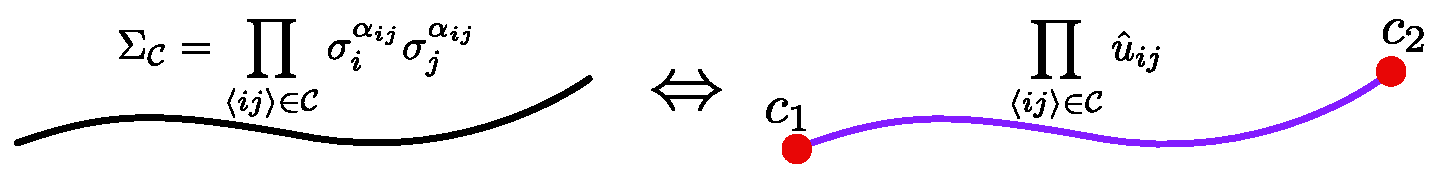
\includegraphics[width=\linewidth]{figures/linking-string.pdf}
    \caption{Two Majorana fermions emerge at the endpoints of a string $\mathcal{C}$. In the fermion representation, the link that connects the two $c$-Majorana fermions is composed of $\mathbb{Z}_2$ gauge-field operators, $\prod_{\anglelr{ij}\in\mathcal{C}} \hat{u}_{ij}$.}
    \label{fig.linking-strings}
\end{figure}

In conclusion, it has been demonstrated that the $\mathcal{M}$-representation is identical to the $\mathcal{S}$-representation. This phenomenon can be understood as follows. Two Majorana fermions, $c_1$ and $c_2$, connected by a string $\mathcal{C}$ of $\mathbb{Z}_2$ gauge-field operators, generate a string operator~\cite{Kitaev}, as illustrated in \autoref{fig.linking-strings}
\[
c_1\lr{\prod_{\anglelr{ij}\in\mathcal{C}} \hat{u}_{ij}}c_2 = \prod_{\anglelr{ij}\in\mathcal{C}}c_i\hat{u}_{ij}c_j \propto \prod_{\anglelr{ij}\in\mathcal{C}}\dimer{i}{j} = \Sigma_{\mathcal{C}}
\]
up to a phase depending on the length of the string $\mathcal{C}$. This relation clearly illustrates that the $c$-Majorana fermions emerge at the endpoints of strings.}

\alert{
\[
\mathcal{S}\lr{\wordfig{0.5}{figures/ij_segment.pdf}} = \mathcal{S}\lr{\wordfig{0.75}{figures/ij_curve.pdf}} = \mathcal{S}\lr{\wordfig{0.8}{figures/ij_segment_1_loop.pdf}} = \cdots
\]

\[
\lsegment{i}{l}\lsegment{k}{i}\lsegment{i}{j} = -\lsegment{i}{j}\lsegment{k}{i}\lsegment{i}{l}
\]
\[
(ic_ic_l)(ic_kc_i)(ic_ic_j) = - (ic_ic_j)(ic_kc_i)(-ic_ic_l)
\]
\[
\mathcal{S}\lr{\wordfig{2}{figures/fermion-braiding_1.pdf}} = -\mathcal{S}\lr{\wordfig{2}{figures/fermion-braiding_2.pdf}}
\]
}

